\subsection{fftMPI}
\emph{fftMPI} is the package we choose to implement to take care of the decomposition. It is installed through the classic set of commands 
\begin{lstlisting}
./configure 
make 
make install
\end{lstlisting}
and produce a couple of different libraries, once for 1D and once for 2D decomposition.
\par
These libraries are accessed through four headers, based on the user needing. In our case we were interested at the remap APIs for 3D arrays, so we called 
\begin{lstlisting} 
remap3d.h .
\end{lstlisting}
Once the header was included we compiled the source code with 
\begin{lstlisting}
-lfft3dmpi
\end{lstlisting}
flag to produce the executable. To link the code is mandatory to use 
\begin{lstlisting}
mpicxx
\end{lstlisting}
or equivalent, since \emph{fftMPI} is written in C++, and not in C. \\
\par
Currently the remap works with floating point data only. Anyway, each datum in a distributed 3D grid can be one or more floating point values. In our case, we employed the method with the parameter
\begin{lstlisting}
nqty = 2
\end{lstlisting}
so that the method select two adjacent floating point values per grid point, and treat them as a single complex number. \\
\par
A pseudo-code to perform array remapping using such package expect the following structure:
\begin{lstlisting}
#include "remap3d_wrap.h" 
remap3d_create(MPI_COMM_WORLD,&remap);

remap3d_set(remap,"collective",cflag);
remap3d_set(remap,"pack",pflag);
remap3d_set(remap,"memory",mflag); 

remap3d_setup(local_input_tiles_coords, local_output_tiles_coords,
              nqty,permute,memoryflag,&sendsize,&recvsize); 
              
FFT_SCALAR *ARR = (FFT_SCALAR *) malloc(remapsize*sizeof(FFT_SCALAR));
FFT_SCALAR *sendbuf = (FFT_SCALAR *) malloc(sendsize*sizeof(FFT_SCALAR));
FFT_SCALAR *recvbuf = (FFT_SCALAR *) malloc(recvsize*sizeof(FFT_SCALAR)); 

/* Fill the array ARR with data */
ARR= ...

remap3d_remap(remap,ARR,ARR,sendbuf,recvbuf); 

remap3d_destroy(remap); 
\end{lstlisting}
As we can see the process is made up of:
\begin{itemize}
\item create the remap container;
\item set options for the remap;
\item define the tiles dimensions and commit the container;
\item execute the remap;
\item destroy the remap container.
\end{itemize}
\par
The options allow users to set the method, used by MPI, to pass the messages. For example, it is possible to decide whether to use collective calls instead of point-to-point communications, or it is possible to select how to pack the messages before sending them.
\par
For further informations, and the source code, refer to~\cite{fftMPI}.


\subsection{Parallel HDF5 Library}
Hierarchical Data Format 5, or HDF5, is widespread scientific data format used by many application to deal with large sets of data~\cite{hdf5}. Parallel Hierarchical Data Format 5, or pHDF5, is the parallelized version for clusters.\par
Designed to store and organize large amounts of data, HDF5 has been originally developed at the National Center for Supercomputing Applications. 
The crucial feature is its ability to store binary dataset in a processor independent fashion, guaranteeing the portability of the data. This allows extremely compact file dimensions, since we are dealing with binary data, and in the same time we can exploit the advantages of ASCII encoding.\par
We could think at the parallel I/O as a bridge between the application and the data, which are stored on memory. In this parallelism our high-level library can be thought as the deck of the bridge. Such deck is built on top of pylons, which is the middleware, the MPI-IO. Our library provide an high level of abstractions, allowing to instruct and tune the middleware to perform the requested operations. On its own MPI-IO deals with organizing access to disk by many processes. Everything is anchored to the ground through foundations, which is our parallel file system.\par
The hierarchical file ordering allows to define a Linux like environment made up of root folder, subfolders, tables, figure, attributes, links and others useful things to maintain the database as readable as possible.\par
\begin{figure}
\begin{center}
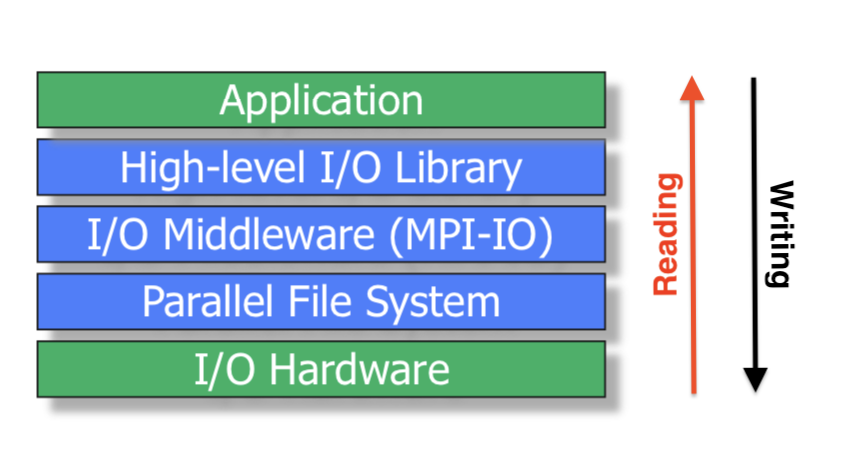
\includegraphics[scale=0.4]{grafici/parallelio}
\caption{Ideal structure of a parallel I/O implementation}
\label{default}
\end{center}
\end{figure}

The price for the high flexibility of such data format is the impossibility to have a plug and play VTK reader. In fact we have to rely on third party software to instruct the VTK tool, in our case Paraview, to inspect the database. \par
We decide to use XDMF3~\cite{xdmf3}, acronym of eXtensible Data Model and Format~3, to generate an XML file to put beside of our HDF5 file, so that Paraview, or any other VTK software, use it to read the database.
Such XML file is automatically generated when the post processor is run. It contains the environmental conditions, such as domain geometry, cell placement, timestep and some instruction to join the velocities data of a cell into a vector. It is used to tell to the VTK reader where and what read from the HDF5 file.
